%%%%%%%%%%%%%%%%%%%%%%%%%%%%%%%%%%%%%%%%%
% Project Synopsis
% LaTeX Template
%
% This template has been downloaded from:
% http://www.vrajport.net
%
% Original author:
% Vaibhavraj Roham (http://www.vrajport.net)
%
% Note:
% The \lipsum[#] commands throughout this template generate dummy text
% to fill the template out. These commands should all be removed when 
% writing assignment content.
%
%
%%%%%%%%%%%%%%%%%%%%%%%%%%%%%%%%%%%%%%%%%

%----------------------------------------------------------------------------------------
%	PACKAGES AND OTHER DOCUMENT CONFIGURATIONS
%----------------------------------------------------------------------------------------
\author{Group ID-06}
\title{Smart Farm using Wireless Sensor Network}
\documentclass[10pt,a4paper]{article}
\usepackage[latin1]{inputenc}
\usepackage{amsmath}
\usepackage{amsfonts}
\usepackage{amssymb}
\usepackage{gensymb}
\usepackage{graphicx}
\usepackage{fancybox}
\usepackage{fancyhdr}
% Margins
\topmargin=-0.45in
\evensidemargin=0in
\oddsidemargin=0in
\textwidth=6.5in
\textheight=9.0in
\headsep=0.25in

\linespread{1.5} % Line spacing

%For the header and footer
\fancypagestyle{plain}{%
\fancyfoot[L]{\emph{Department of Computer Engineering, S.R.E.S' College of Engineering, Kopargaon}} % except the center
\fancyfoot[R]{\thepage}
\renewcommand{\headrulewidth}{0.4pt}
\renewcommand{\footrulewidth}{0.4pt}
}

\pagestyle{fancy}
\rhead{\emph{Smart Farm Using Wireless Sensor Network}}
\lhead{}
\fancyfoot[LO,LE]{\emph{Department of Computer Engineering,  S.R.E.S's College of Engineering, Kopargaon.}}
\cfoot{}
\fancyfoot[RO, RE]{\thepage}
\renewcommand{\headrulewidth}{0.4pt}
\renewcommand{\footrulewidth}{0.4pt}
%For the header and footer Over
\begin{document}
%\tableofcontents
%\newpage
\begin{center}
\begin{huge}
\textbf{PROJECT SYNOPSIS}
\end{huge}
\end{center} 
\textbf{Project Title : } ``Smart Farm Using Wireless Sensor Network" \\
\textbf{Year : } 2015-2016 \\
\textbf{Group ID : } 06
\begin{large}
\section{Keywords}
\end{large}

\quad
\textit{Automation, Farming, Technology, Wireless Sensor Network, ZigBee, XBee, BeagleBone, Router, Access Point, Solar Plates, Android, Database, Server, Temperature, CO\ensuremath{_2}, Humidity, Intrusion, Remote, Wireless, Internet, Sensor, Agriculture, Green House, Controller, Sink, Sensing Node, Node, Gateway, Monitoring, Operating.} 
 
\begin{large}
\section{Project Description}
\end{large}
\quad
Automation is the use of machines, control systems and information technologies to optimize productivity in the production of goods and delivery of services. Automation is the answer to India's pursuit for being a world-class industrial competitor. The Indian farms are slowly beginning to feel the stimulus for the instrumentation, control and automation industry. Indian automation is advancing at a fast pace, yet it is one area that can never be achieved and admired, it is something that needs constant innovation and identification of trends in technology, and the innovations that thrust the implementation of automation in other countries. India, as one of the world's fastest growing economies based on agriculture and farming, has not taken to technology at a rather quick pace. A large number of farmers in India are turning towards the construction of Green Houses. \\

\quad
To make the automation system work properly with in an ultra modern and a big green houses, several measurement points are required to trace down the local climatic condition parameters at different locations. Using cabling for monitoring would make the measurement system expensive, vulnerable,
and also the measurement points are difficult to relocate. Due to these facts, a WSN consists of small-size wireless sensor nodes with radio and sensors are more cost efficient and practical option to build the required parameters measurement system \cite{1}. \\

\quad
In an agriculture field the farmers or the agriculture expert can observe the measurements periodically like temperature and humidity levels inside the fields, from the web simultaneously. Moreover, when a critical change in one of the measurements occurs, then the farmer will be notified via e-mail, SMS and Android Mobile Application. Thus by this way, the farmer will be acknowledged in such a needy situation at an earliest time possible and may be able to prevent possible damaging effects of those changes \cite{1}. A wireless sensor network consists of a large number of nodes which are deployed densely in an agriculture land for various physical parameters to be measured or monitored. Each of these nodes gathers the data and route this information back to a coordinator. As the positions of individual nodes are not predetermined, then that network must possess self-organizing capabilities. Thus Cooperation among these nodes is the dominant feature of this type of networks, where groups of nodes cooperate to disseminate the information which is already gathered in their vicinity to the user. \\

\quad
In Green House the controller node will be connected to internet by which it can dump all the readings into web-server periodically. Now, the farmers android mobile application and web application will be connected to web-server, from where farmer can continuously monitor the levels of , Temperature and humidity. 
\begin{large}
\section{Scope}
\end{large}
\begin{enumerate}
\item The system will be design in way to ensure that,
\begin{enumerate}
\item Farmers can remotely monitor the green house climate parameters.
\item Operating farm equipments remotely via web application.
\item Analysis of climate parameters for detecting changes.
\item Acknowledging the farmer on instant changes in climate parameters.
\end{enumerate}
\item Location based Weather Information to farmer.
\item Multi-Language support for software application to ease of use by farmer. 
\end{enumerate}

\begin{large}
\section{Objective}
\end{large}
Objective of the project are,\\
\begin{enumerate}
\item To make use of technology in farming.
\item To reduce the manpower of individual monitoring and analyzing parameters.
\item To minimize the traditional methods of farming and make use of technology in farming and make the farming process easy.
\item Analysing climate parameters and pretending some actions accordingly to improve the crop production.
\item Remote monitoring of the farm and it's climate parameters.
\end{enumerate}


\begin{large}
\section{Review of Conference/Journal Papers and Relevant Theory}
\end{large}

\quad
This section contains the Literature review and the theory about the project. 

\subsection{Agriculture Field Monitoring and Analysis using Wireless Sensor Networks for improving Crop Production}

\quad
The purpose of this is to design and develop an agricultural monitoring system using wireless sensor network to increase the productivity and quality of farming without observing it for all the time manually. Temperature, humidity and carbon dioxide levels are the most important factors for the productivity, growth, and quality of plants in agriculture. So this system periodically measures these parameters inside the fields, thus the farmers or the agriculture experts can observe the measurements from the web simultaneously. Moreover, when a critical change in one of the measurements occurs, then the farmer will be intimated via mobile text message and e-mail by an agriculture expert. \cite{1}
 
\subsection{Wireless Sensor Network for Precise Agriculture Monitoring}

\quad
Precision Agriculture Monitor System (PAMS) is an intelligent system which can monitor the agricultural environments of crops and provides service to farmers. PAMS based on the wireless sensor network (WSN) technique attracts increasing attention in recent years. The purpose of such systems is to improve the outputs of crops by means of managing and monitoring the growth period. This paper presents the design of a WSN for PAMS, shares our real-world experience, and discusses the research and engineering challenges in implementation and deployments. \cite{2}

\subsection{Design and Development of Precision Agriculture System Using Wireless Sensor Network}

\quad
Crop farming in India is labour intensive and obsolete. Farming is still dependent on techniques which were evolved hundreds of years ago and doesn't take care of conservation of resources. The newer scenario of decreasing water tables, drying up of rivers and tanks, unpredictable environment present an urgent need of proper utilization of water. We have the technology to bridge the gap between water usage and water wastage. Technology used in some developed countries is too expensive and complicated for a common farmer to understand. Our project is to give cheap, reliable, cost efficient and easy to use technology which would help in conservation of resources such as water and also in automatizing farms. We proposed use of temperature and moisture sensor at suitable locations for monitoring of crops. The sensing system is based on a feedback control mechanism with a centralized control unit which regulates the flow of water on to the field in the real time based on the instantaneous temperature and moisture values. The sensor data would be collected in a central processing unit which would take further action. Thus by providing right amount of water we would increase the efficiency of the farm. The farmer can also look at the sensory data and decide course of action himself. We have made the interface of our project keeping in view the educational and financial background of average Indian farmer. \cite{3}

\subsection{Wireless Sensor Networks: Apple farming in Northern India}

\quad
Wireless Sensor Networks (WSN) is an emerging technology that has spread rapidly into various multidisciplinary fields. Recently the agriculture and farming industry has diverted their attention to WSN, seeking this cost effective technology to improve its production and enhance agriculture yield standard. This paper presents a brief survey of WSN and its uses in agricultural practices. Main emphasis of our study is on the use of WSN for apple farming and precision agriculture. Our paper presents a detail report on the land area used for apple farming in India. This paper also discusses some of the challenges in using WSN for apple farming. Despite of having vast area of land for cultivation, detailed finding of our study reports the poor yield (production per unit area) of apples in India. Our survey report also suggests the use of WSN for increasing the apple production. \cite{4}

\subsection{An environment monitoring system for precise agriculture based on wireless sensor networks}

\quad
To solve the problems occurring in the traditional precision agriculture such as poor real-time data acquisition, small monitoring coverage area, excessive manpower requirement etc., this paper designs and deploys an environment monitoring system for precise agriculture based on wireless sensor networks in a red bayberry greenhouse located on a hillside. This system can automatically collect the temperature, humidity, illumination, voltage and other parameters of the deployment zone, and transmit the data to the remote server via GPRS in real time. This system also includes a web-based platform integrated with Google Maps to release the greenhouse environmental status and provide real-time voice and SMS alarm service. Since the experimental area is lack of mains supply, the system is powered by solar and storage batteries. The experiment result shows that the low-cost system has strong scalability, and can provide real-time, stable and accurate service for precise agriculture. \cite{5}
 
\subsection{Study on Precision Agriculture Monitoring Framework Based on WSN}

\quad

The wireless sensor networks (WSN) is one of the most significant technologies in the 21st century. In recent years, achievements in micro-sensor technology and low-power electronics make WSN become into realities in applications. This paper describes a real-deployment of WSN based greenhouse management which is designed and implemented to realize modern precision agriculture. The proposed system can monitor the greenhouse environments, control greenhouse equipment, and provide various and convenient services to consumers with hand- held devices such as a PDA living a farming village. This paper discusses the advantages of using management strategy along wireless sensor-actor network technology for such cost-effective and environmental friendly greenhouse management. \cite{6}

\subsection{A\ensuremath{^2}S: Automated Agriculture System based on WSN}

\quad
This paper describes the results of real deployment of A\ensuremath{^2}S which consists of WSN(Wireless Sensor Network) to monitor and control the environments and a management sub-system to manage the WSN and provide various and convenient services to consumers with hand-held devices such as a PDA living a farming village. The WSN were deployed in greenhouses with melon and cabbage in Dongbu Handong Seed Research Center. A\ensuremath{^2}S was used to monitor the growing process of them and control the environment of the greenhouses. We acquired valuable experiences and ideas from this real deployment and operation of A\ensuremath{^2}S and believe that they can be useful in consumer electronics field such as home network as well as automated agriculture field. \cite{7}

\subsection{Smart Farm: Extending Automation To The Farm Level}

\quad 
 With the advent of technology, the world around us is getting automated. Automatic systems are being favored over manual systems, as they are energy efficient and minimize the need for tedious manual labor. With agriculture being the primary economic sector of India and other developing countries, it is essential to automate it in order to increase efficiency. A typical farm requires a lot of labor. Automation can proficiently moderate the amount of manual labor, and make farming easier and faster, leading to more agricultural growth. The concept of automation is extended to the agricultural farms and farm houses. Numerous aspects of the farm are automated, which include auto-irrigation cycles and secure temperature controlled enclosures for livestock and farm products. In our paper, we implement automatic lighting system, auto-sprinkler system, in-house temperature control and security for farm houses. As temperature and motion sensitive devices will only work when required, such a system conserves energy effectively. The paper also presents features to enhance the security of the farm. Energy efficient farm automation is the need of the hour in an agro-based economy. \cite{8}


\subsection{BeagleBone Black}

\quad
The most important part of the system is \textit{Wireless Sensor Network (WSN)}. For implementing the Wireless Sensor Network we require various devices and sensors. Below is the brief description of parts of WSN. \cite{9}

\quad
It is the open-source development board with RAM of 512 MB, the processor clock to 1 GHz, and it adds HDMI and 2 GB of eMMC flash memory. The BeagleBone Black also ships with Linux kernel 3.8, upgraded from the original BeagleBone's Linux kernel 3.2, allowing the BeagleBone Black to take advantage of Direct Rendering Manager (DRM).\\
The BeagleBone Black is the newest member of the BeagleBoard family. It is a lower-cost, high-expansion focused BeagleBoard using a low cost Sitara XAM3359AZCZ100 Cortex A8 ARM processor from Texas Instruments. It is similar to the Beaglebone,but with some features removed and some features added. The table below gives the high points on the differences between the BeagleBone and BeagleBone Black.\cite{5}

\begin{figure}[hbtp]
\centering
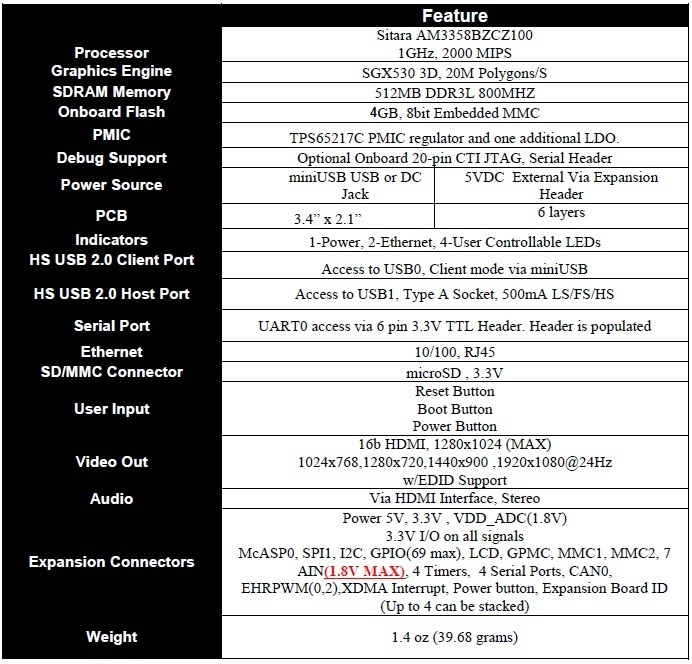
\includegraphics[scale=0.78]{Features.jpg}
\caption{BeagleBone Black Specifications}
\end{figure}

\subsection{ Zigbee Device (XBee)}

\quad
According to Digi ``XBee modules are embedded solutions providing wireless end-point connectivity to devices. These modules use the IEEE 802.15.4 networking protocol for fast point-to-multipoint or peer-to-peer networking. They are designed for high-throughput applications requiring low latency and predictable communication timing." So basically XBee is Digi's own Zigbee based protocol. They are fairly easy to use in wireless modules. \cite{10}

\begin{figure}[hbtp]
\centering
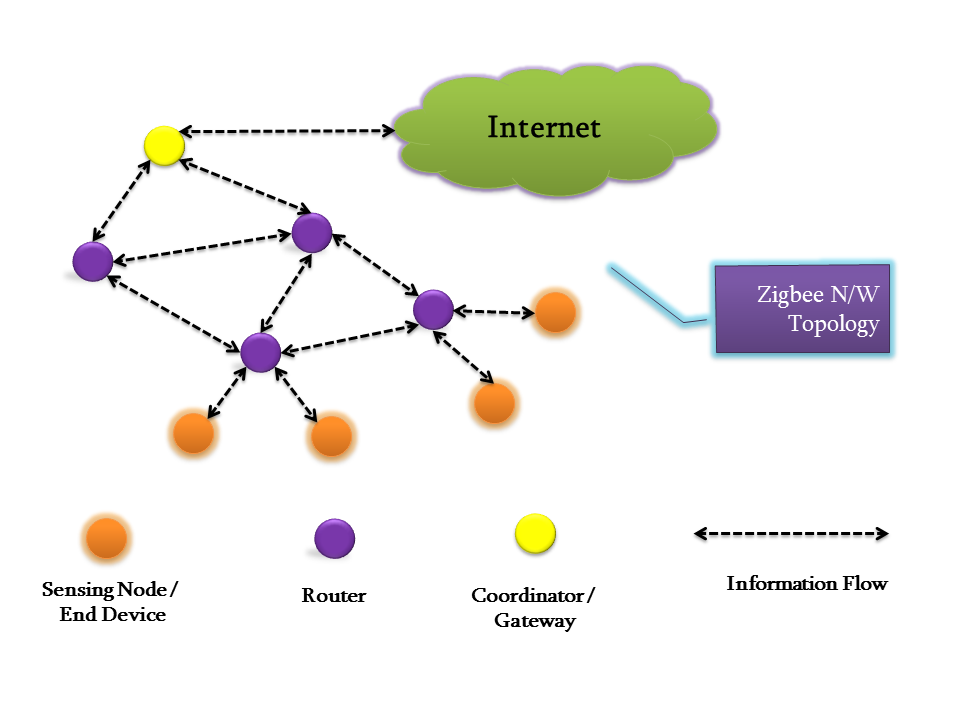
\includegraphics[scale=0.5]{present.png}
\caption{Working of Zigbee Devices}
\end{figure}


\quad 
ZigBee is a specification for a suite of high-level communication protocols used to create personal area networks built from small, low-power digital radios.ZigBee is typically used in low data rate applications that require long battery life and secure networking (ZigBee networks are secured by 128 bit symmetric encryption keys.) ZigBee has a defined rate of 250 kbit/s, best suited for intermittent data transmissions from a sensor or input device.
Applications include wireless light switches, electrical meters with in-home-displays, traffic management systems, and other consumer and industrial equipment that requires short-range low-rate wireless data transfer.The technology defined by the ZigBee specification is intended to be simpler and less expensive than other wireless personal area networks (WPANs), such as Bluetooth or Wi-Fi.\cite{6}


\begin{large}
\section{System Architecture/ Module Details}
\quad \quad\quad This section contains the implementation details of the exiting system and proposed system 
\end{large}


\subsection{Existing System}

\quad
This section contains the information and highlighting details about the existing system which are being used.
\begin{itemize}
\item \textbf{Libelium World :} 

\textit{``Smart Agriculture: Monitoring Greenhouse Conditions To Develop New Products"}


\quad
Flores en la mesa reserved an area and a greenhouse structure for its sensor installations. The system includes Waspmote Plug and Sense Agriculture nodes installed in a greenhouse, to measure factors such as temperature, humidity, solar radiation, and luminosity over a large cultivated surface.The greenhouse measures 12 x 5 m - 60 m, with two auxiliary plantations (interior and exterior).Some of nodes are equipped with solar panels to harvest energy, and communicate via XBee and 3G modules.

\begin{figure}[hbtp]
\centering
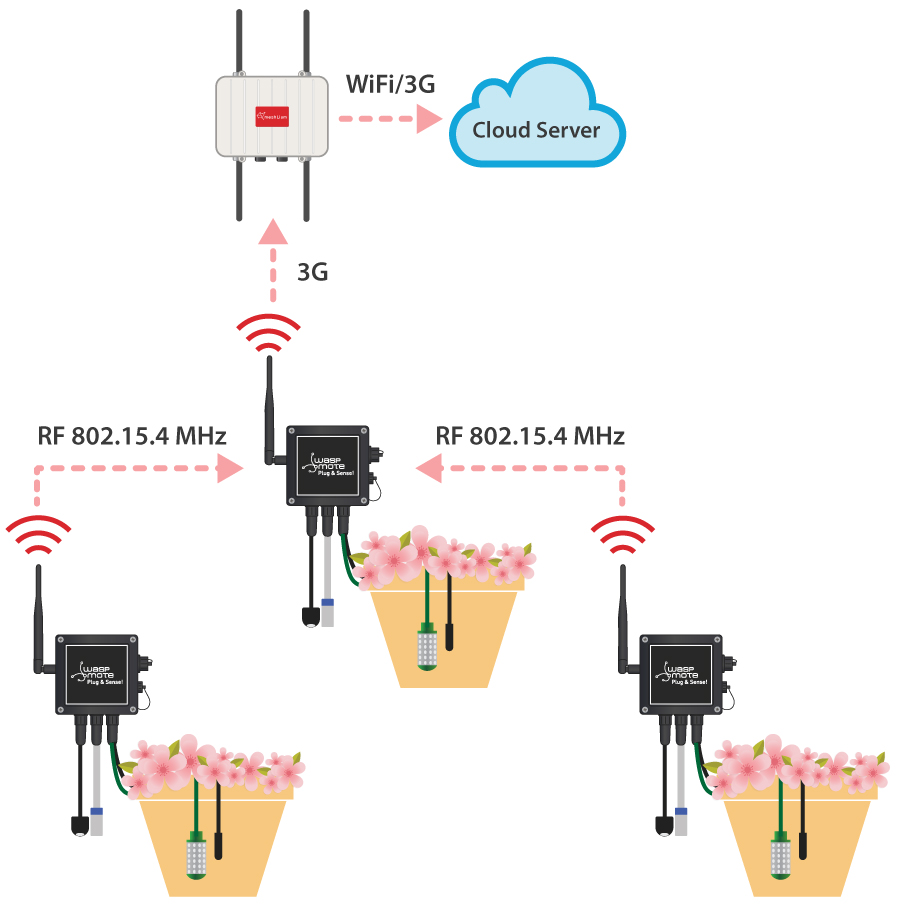
\includegraphics[scale=0.4]{FM_diagram.jpg}
\caption{Flores en la mesa Schema Architecture}
\end{figure}

\quad
Sensor nodes have direct access to power, with probes situated at various levels, from the ground to the greenhouse ceiling, in position to capture and measure the different parameters. Waspmote Plug and Sense Agriculture boards are fully charged and programmed, from the factory. To connect them, Libelium created a XBee network with star topology. Two of the nodes send data periodically every 15 minutes to the central node. This node collects the data along with its own sensor data and sends it via 3G to a server.




\item \textbf{Jain Integrated Automation Systems}

\quad 
Manual operation of the routine practices in agriculture requires lot of attention and care. Also it is difficult to perform desired jobs efficiently and precisely. Ultimately this may result in lower crop production, non-uniform growth and poor quality.

\quad
Jain Irrigation provides various automation solutions to overcome these problems and to maximize the yields. Automation provides a faster, precise and reliable operation. Jain Irrigation has the complete range to suit specific requirements in agriculture, landscape, precision farming, Green houses and nurseries, lift irrigation etc.

\begin{figure}[hbtp]
\centering
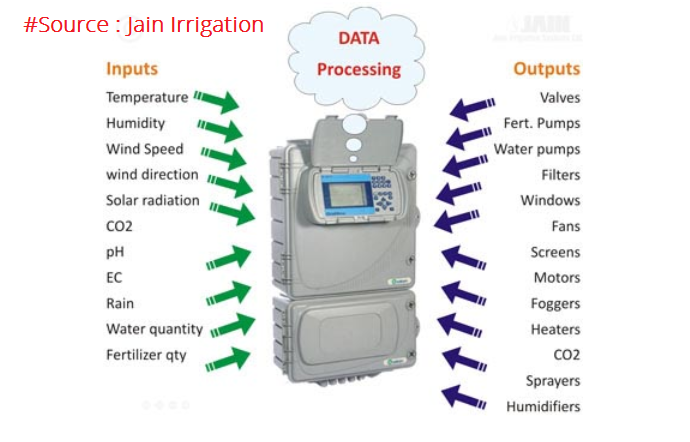
\includegraphics[scale=0.6]{jain2.PNG}
\caption{Machine Layout of Jain Irrigation}
\end{figure}

\end{itemize}



\subsection{Proposed System Module Details}

\quad
This section contains the block diagram and the details about the modules we are going to use. 

\begin{itemize}
\item \textbf{ Proposed System Architecture}

\quad
  As shown in Figure 5, Details about the Proposed System Architecture are,

\begin{figure}[htbp]
\centering
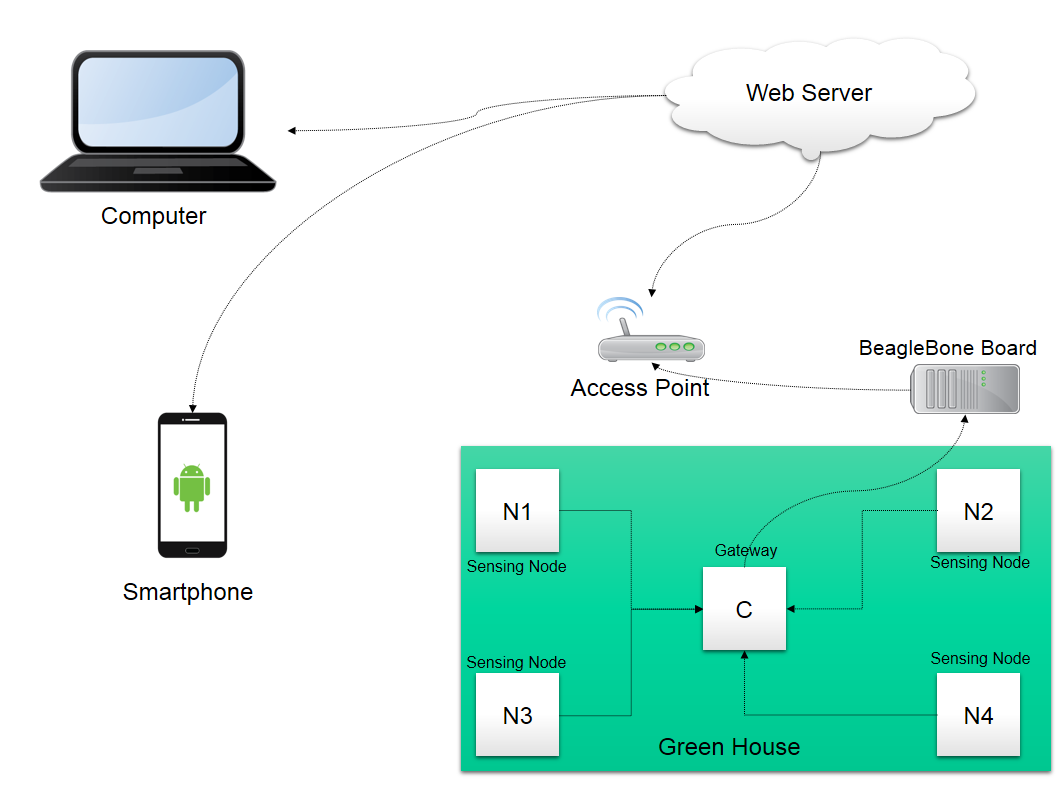
\includegraphics[scale=0.3]{s1.png}
\caption{System Architecture}
\end{figure}

Various devices/blocks are present in architecture, following is the brief description of it,

\begin{enumerate}
\item \textbf{Sensing Node : }  

\quad
Sensing node is the xbee (Zigbee) radio device on which various sensors are mounted. Sensing node is connected to controller/gateway. It will sense the various readings at specific interval and forward it to gateway.\cite{5}

\item \textbf{Gateway : }

\quad
Gateway is a xbee (Zigbee) wireless device which will accept the values from various sensing nodes. Gateway is connected to BeagleBone Board which is capable of processing of all the values. All the readings are forwarded to BeagleBone for processing by gateway.


\item \textbf{BeagleBone Board : }

\quad
BeagleBone is processor embedded board which is capable of processing the input also to connect external networks. BeagleBone is connected to Access Point for Internet connectivity. BeagleBone access the web-server and dump all the values in database using web-server API.\cite{5}


\item \textbf{Access Point : }

\quad
Access Point is the hotspot for the Internet connectivity for various devices. It will provide wireless internet connectivity to BeagleBone.  

\item \textbf{Web-Server : }

\quad
Web-Server is used to store the readings forwarded by BeagleBone Board from Green House. It is capable of analyzing the parameters and predict he situation accordingly. If uncertain conditions occurs it is capable of generating alert's such as push notification for android mobile application, Sending SMS to farmer's mobile etc. 

\quad
Also, The web application for real-time analysis, monitoring and controlling will be deployed on web-server. This application will be directly accessible from anywhere by using security credentials.

\item \textbf{Computer/Desktop/Mobile : }

\quad
This are the standard monitoring devices from where we can monitor the Green House from any remote location. In future advancement we can connect display directly in the Green House to get real time statistics.
\end{enumerate}
\item \textbf{Project Modules}

\quad
As shown in Figure 6, describes the modules of our proposed system.

\begin{figure}[hbtp]
\centering
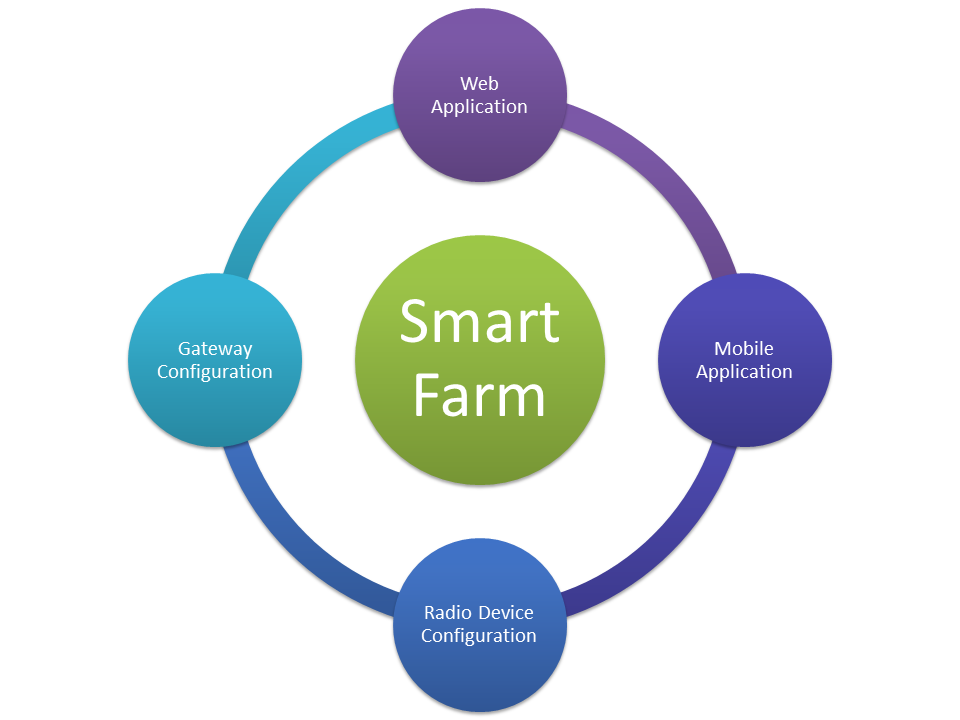
\includegraphics[scale=0.5]{Diagrams.png}
\caption{Project Modules }
\end{figure}
\begin{enumerate}
\item \textbf{Radio Device Configuration:}

\quad
In this module we will configure the radio devices with sensors and add network parameters to communicate with other devices in network.

\item \textbf{Gateway Configuration:}

\quad
	Configuration of Gateway Device i.e. BeagleBone Device with the radio devices and access-point to store the readings in database.

\item \textbf{Web Application:}

\quad
	Web Application will be used to handle the environment parameters and analyse them and acknowledge the farmers. Devices can be operated remotely using web application.

\item \textbf{Mobile Application}

\quad
	We can monitor the parameters and operate the devices remotely from mobile application.

\end{enumerate}
\end{itemize}
\begin{large}
\section{System Requirements}
\end{large}
Hardware and Software requirements for the system are stated below,
\begin{large}
\subsection{Hardware Requirements}
\end{large}
\begin{enumerate}
\item BeagleBone Black Board (Sitara)
\item XBee Radio Device (ZigBee)
\item CO\ensuremath{_2}, Temperature and Humidity Sensor
\item Solar Plates
\item Connection Cables 
\item Batteries
\item Router/Access Point
\item Computer ( Minimun Configuration )
\item Android Smartphone
\item LED Display

\end{enumerate}
\begin{large}
\subsection{Software Requirements}
\end{large}
\begin{enumerate}
\item LAMP Web-Server (Apache, PHP, MySQL)
\item XCTU Utility for XBee Configuration
\item Android Studio 
\item Web Browser(Mozilla Firefox)
\item PHP and MVC Framework 
\end{enumerate}

\newpage
\section{Project Execution Plan}

\quad
 Figure 7, 8, 9 describes the schedule for project development and also highlights all the tasks to be carried out along with their duration and dependency to accomplish the task.

\subsection{Execution Timeline for Phase I}
\begin{figure}[hbtp]
\centering
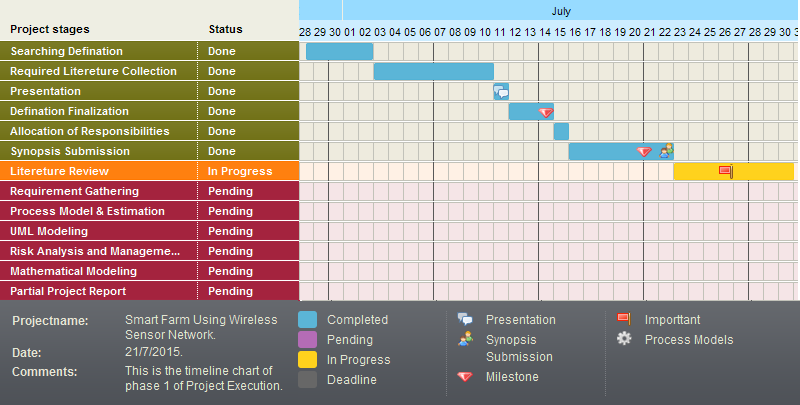
\includegraphics[scale=0.760]{1.png}
\caption{Project Execution Timiline (June-July) }
\end{figure}
\begin{figure}[hbtp]
\centering
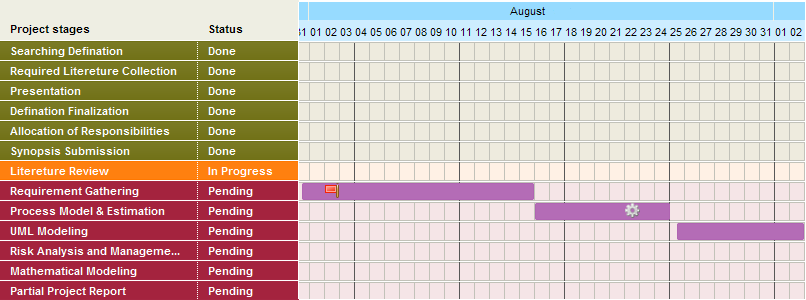
\includegraphics[scale=0.760]{2.png}
\caption{Project Execution Timiline (August) }
\end{figure}
\begin{figure}[hbtp]
\centering
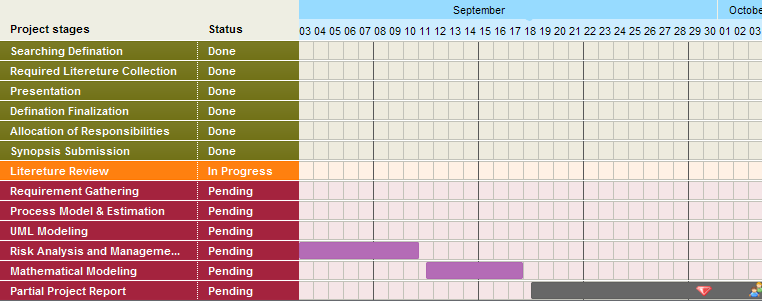
\includegraphics[scale=0.760]{3.png}
\caption{Project Execution Timiline (September - October) }
\end{figure}

\newpage %Replace with landscape Image

\section{Application/Usefulness}
\begin{enumerate}
\item Low cost solution for implementation and affordable to farmers. 
\item Wireless communication technology so easy to use and move to any remote location.
\item Automatic time provisioning alerts on instant climate parameter variations.
\item Analysis of various environmental/climate parameters like CO\ensuremath{_2}, temperature and humidity.
\item Use of renewable energy source i.e. Solar Energy to power the devices in day time.
\item Remote operations on Green House Devices.
\end{enumerate}
\begin{large}
\section{Conclusion}
\end{large}

\quad
In farming Temperature, Humidity and CO\ensuremath{_2} are the most essential parameters. The growth of crops is mainly depend on these three parameters. Currently farmers don't have any system which will show realtime levels of these parameters. Even farmer don't know when humidity is increased or CO\ensuremath{_2} level increased in his green house, because of it crop production gets affected. The proposed system is going to monitor these changes periodically and take an action automatically or pretend the required action to the farmer. System will have a provision to visualize the graphical representation of all the streaming data from the green house. Later on farmer can operate the devices from remote location by using its smart phone.

\addcontentsline{toc}{section}{\hspace{6mm}REFERENCES}
\newpage
\begin{thebibliography}{2}

\bibitem{1} B. Balaji Bhanu, K. Raghav Rao, J. V. N. Ramesh, Mohammed Ali Hussain, ``Agriculture Field Monitoring and Analysis using Wireless Sensor Networks for improving Crop Production", IEEE, 2014. Access Date: 09/07/2015.

\bibitem{2} Shining Li, Jin Cui,  Zhigang Li,"Wireless Sensor Network for Precise Agriculture Monitoring", 2011, China. Access Date: 09/07/2015.

\bibitem{3}SR Nandurkar, TR Thool, RC Thool, "Design and Development of Precision Agriculture System Using Wireless Sensor Network". Access Date: 09/07/2015.


\bibitem{4}N Rajput, N Gandhi, "Wireless Sensor Networks: Apple farming in Northern India", 2012, IEEE. Access Date: 09/07/2015.

\bibitem{5}Jianfa Xia, Zhenzhou Tang, Xiaoqiu Shi, Lei Fan, Huaizhong Li ,"An environment monitoring system for 
precise agriculture based on wireless sensor networks", 2011, IEEE. Access Date: 09/07/2015.

\bibitem{6} Xuemei Li,Yuyan Deng, Lixing Ding , "Study on Precision Agriculture Monitoring Framework Based on WSN 
",2010, China. Access Date: 09/07/2015.

\bibitem{7} Seong-eun Yoo, Jae-eon Kim, Taehong Kim, Sungjin Ahn, Jongwoo Sung, Daeyoung Kim,"A2S: Automated 
Agriculture System based on WSN", IA, Korea. Access Date: 09/07/2015.

\bibitem{8} Drishti Kanjilal, Divyata Singh, Rakhi Reddy, Prof Jimmy Mathew,"Smart Farm: Extending Automation To 
The Farm Level ", IJSTR, 2014. Access Date: 09/07/2015.

\bibitem{9} ``BeagleBone Black", https://en.wikipedia.org/wiki/BeagleBoard\#BeagleBone\_Black. Access Date: 15/07/2015.

\bibitem{10} ``Digi's Zigbee", https://www.sparkfun.com/pages/xbee\_guide. Access Date: 15/07/2015.

\bibitem{11} Thomas Ummels, ``Project Scheduling Tool",  https://www.tomsplanner.com/
 
\end{thebibliography}


\newpage

\begin{Large}
\textbf{Group Members}
\end{Large}

\begin{table}[hbp]

\begin{tabular}{|p{0.5in}|p{1.0in}|p{3.0in}|p{1.3in}|}  \hline 		
\centering \textbf{\#} &  \centering\textbf{Roll No} &  \centering\textbf{Student Name} &  \textbf{Signature}  \\ \hline 
%Row 1
\centering 1 & \centering 133 & \centering Vaibhavraj Roham & \  \\ \hline 
%Row 2
\centering 2 & \centering 123 & \centering Abhijeet Patil & \  \\ \hline
%Row 3
\centering 3 & \centering 132 & \centering Shubham Raut & \  \\ \hline 
%Row 4
\centering 4 & \centering 134 & \centering Prasad Rupnar & \  \\ \hline  
\end{tabular}
\end{table}

\ \\ \\ \\ \\ \\ \\ \\ \\ \\ \\ \\
\begin{flushleft}
\textbf{Project Co-ordinator and Project Guide}\quad\quad\quad\quad\quad\quad\quad\quad\quad\quad\quad \textbf{Head of Computer Department}
\end{flushleft}
\quad\quad\quad\quad\quad\textit{(Dr. A. B. Pawar)}
\quad\quad\quad\quad\quad\quad\quad\quad\quad\quad\quad\quad\quad\quad\quad\quad\quad\quad\quad\quad 
\textit{(Prof. D. B. Kshirsagar)}

\end{document}